\chapter{2D simulation}

In order to create an accurate model of the LIM system, it is important to understand how it functions. Previous reports have given some insight into this, but none of them have demonstrated a LIM robot that can climb consecutive steps. Wilson performed a simple simulation of a LIM robot in Algodoo, and concluded that the robot would need LIMs for the rear wheels in order to support consecutive stair climbing \citep{Wilson-2013}, however all of the subsequent projects simply used a dragging tail instead of rear wheels. There is a need to resolve this inconsistency in past work, and to gain insight into the function of the LIM system. To do this, another 2D simulation using Algodoo is performed.

\section{Limitations}

Algodoo is a two dimensional physics sandbox \citep{Algodoo}. Initial testing with the software showed that limitations on the physics engine prevent accurate simulation of gears with teeth at a centimetre scale. This means it is impossible to accurately simulate a LIM device at the scale that they would be used in reality. The simulation can be scaled up to avoid this issue. However, this prevents an accurate simulation of the kinematics of the system.\\

Additionally, it was found that Algodoo does not allow for the accurate simulation of an electric motor. In a typical electric motor, the available torque will decrease as the speed increases. This nuance is not present in Algodoo, so it cannot be used to provide an accurate simulation of the motor requirements. Despite these limitations. Algodoo is still useful as a tool to roughly test the motion of LIMs, and to determine how it would interact with steps. The advantage of Algodoo over other simulation methods is its ease of use, it only takes a few minutes to build a LIMed robot in Algodoo.

\section{Configuration}


To improve the accuracy of the Algodoo physics engine, the simulation frequency is set to 1200 and all objects are scaled up 100 times. A basic LIM system with a dragging tail is set up, using gear and wheel dimensions from \cite{Powrie-2019}, shown in Figure \ref{algo-model}.

\begin{figure}[h]
	\centering
	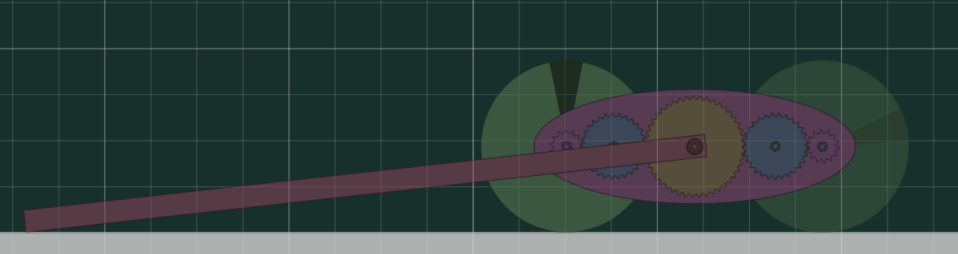
\includegraphics[width=0.8\textwidth]{algo-model}
	\caption{Initial Algodoo LIM system}
	\label{algo-model}
\end{figure}
\section{Observations}

\subsection{Rear wheels}

Simulations suggest that rear wheels are not necessary for successful consecutive stair climbing. If the motor torque is sufficient, the LIM will be able to climb steps with only a dragging tail for counter torque. It should be noted that adding a motorised rear wheel, with or without LIMs, does provide a supporting force to the front LIMs during flipping motion, so if the frontal motor cannot provide sufficient torque, rear wheels should be considered in the design.

\subsection{Mounting obstacles}

There are three ways in which a LIM can mount an obstacle after flipping up to it. The first is that the wheel collides directly with the obstacle, shown in Figure \ref{algo-case-wheel}. This happens when the obstacle is taller than a certain threshold based on the geometry of the LIM, and can result in the wheel bouncing off of the obstacle and failing to pull itself up. In this case a controller may be used to limit the speed of the flipping motion to ensure that the wheel is not going fast enough to bounce off the obstacle when it collides. \\

\begin{figure}[h]
	\centering
	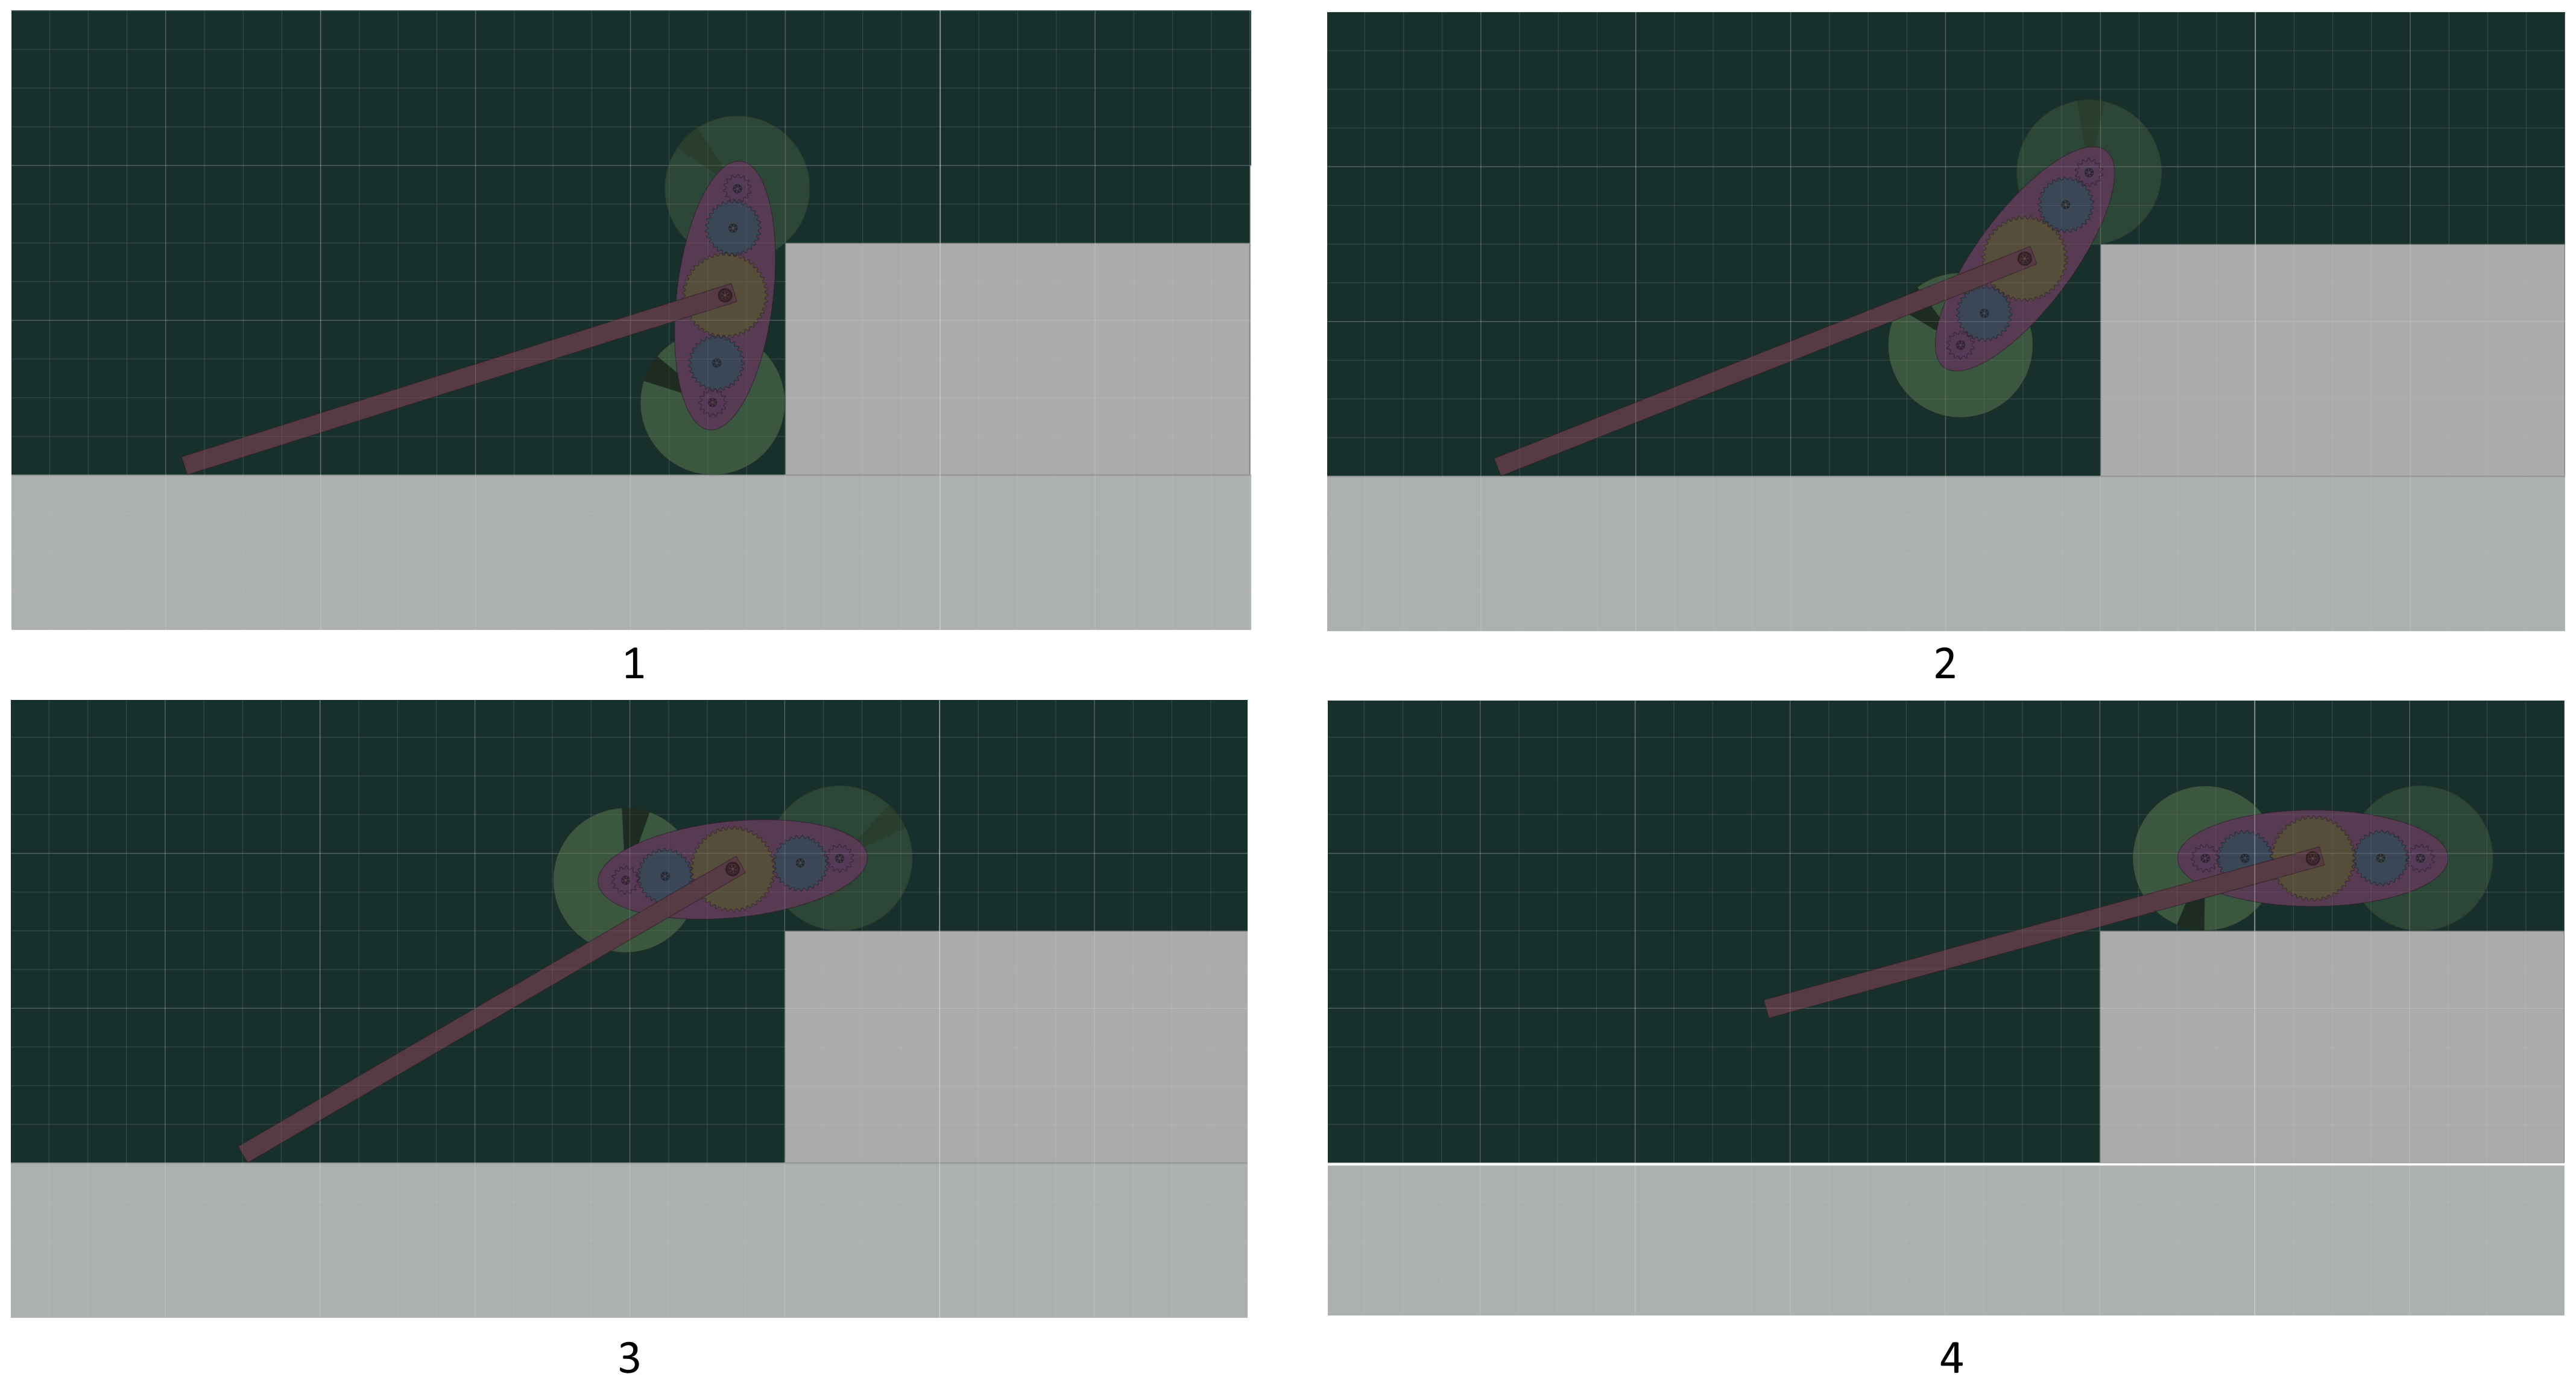
\includegraphics[width=0.8\textwidth]{algo-case-wheel}
	\caption{LIM climbing with wheel contact}
	\label{algo-case-wheel}
\end{figure}

The second way is that the LIM frame collides with the obstacle and mounts it, then the LIM continues to rotate until the wheel makes contact with the surface of the obstacle to pull the robot forward. This case is shown in Figure \ref{algo-case-frame}. Note that the LIM frame can slip on the edge of the obstacle, which may result in failure to climb. \\

\begin{figure}[h]
	\centering
	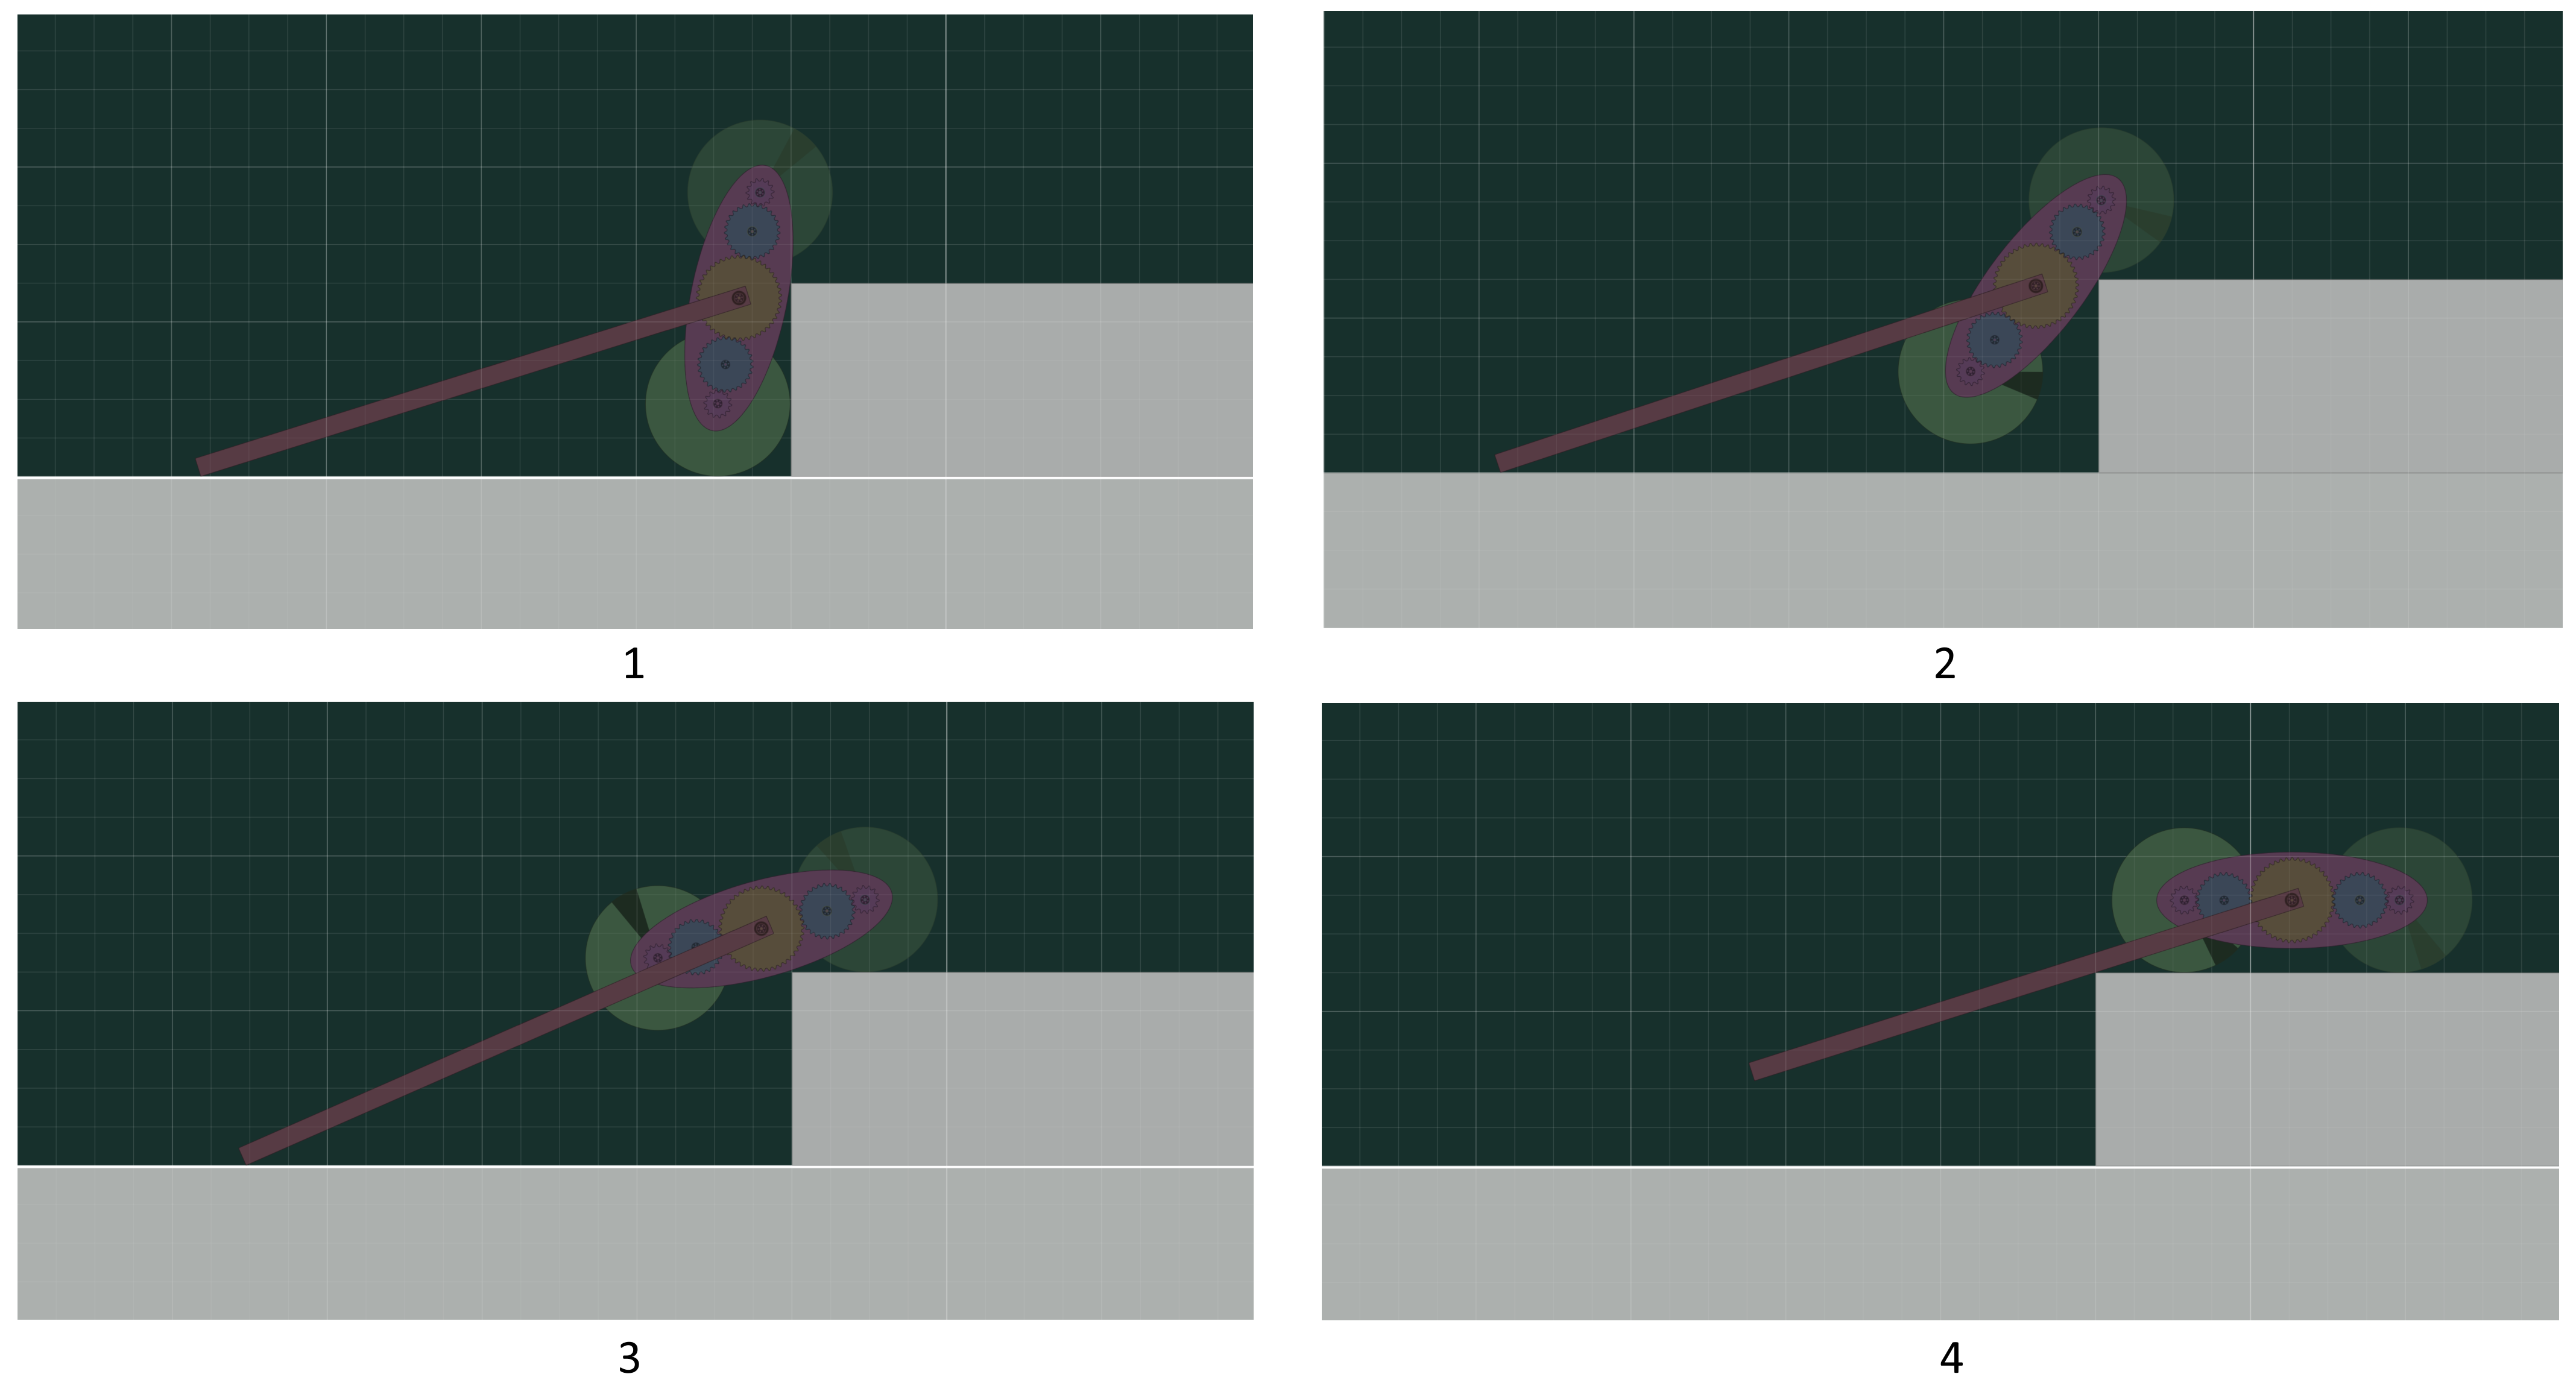
\includegraphics[width=0.8\textwidth]{algo-case-frame}
	\caption{LIM climbing with LIM frame contact, note how the contact point slips between 1 and 2}
	\label{algo-case-frame}
\end{figure}

The third way is that the body of the robot, presented here as an extension of the tail, will mount the obstacle. This is shown in Figure \ref{algo-case-body}. When the body has beached onto the obstacle, seen in Figure \ref{algo-case-body}.2, there is nothing resisting the motion of either the wheels or the LIM, so they can accelerate quite quickly. If they move too fast, the wheel can bounce off the obstacle when it makes contact, dislodging the body so that it falls back down to the initial position. \cite{Buchanan-2018} found that his Ascender followed this motion, which caused it to fail many of its climbing tests. He mentions that this can be avoided by moving the LIM axle to the end of the body, so that the body does not protrude beyond the LIM frame during climbing motion.\\

\begin{figure}[h]
	\centering
	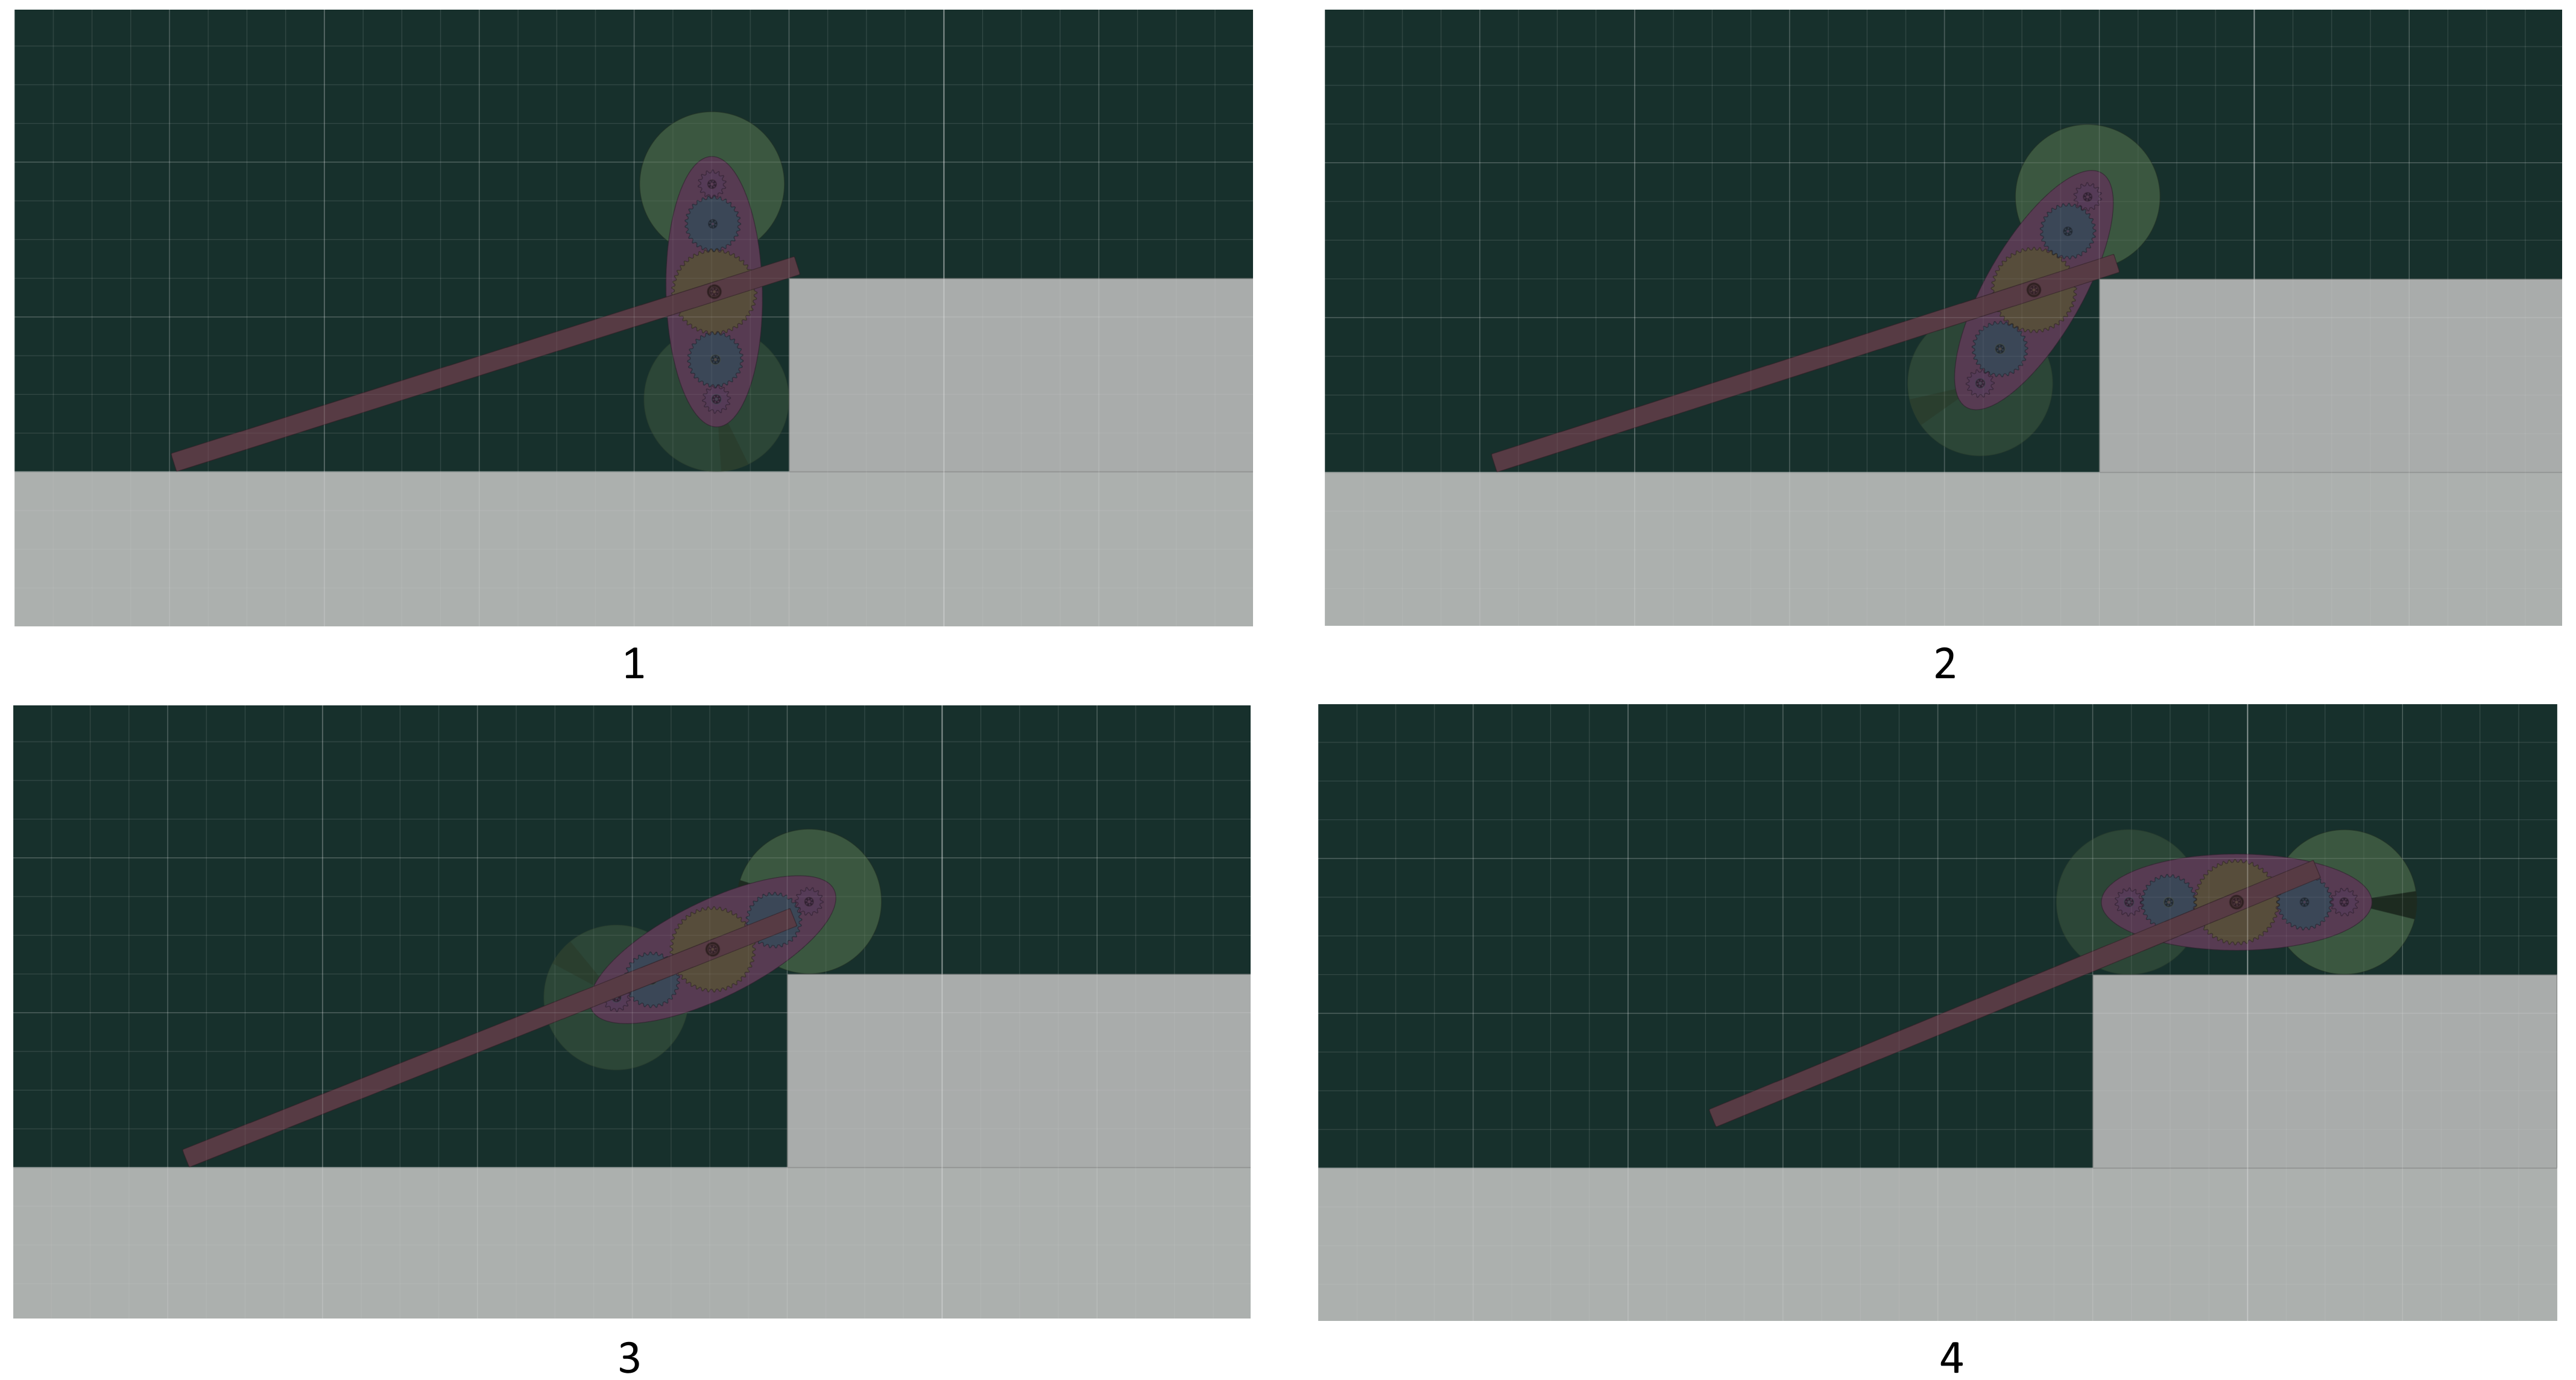
\includegraphics[width=0.8\textwidth]{algo-case-body}
	\caption{LIM climbing with robot body contact}
	\label{algo-case-body}
\end{figure}

Each of these climbing methods has its flaws, however the case where the LIM frame collides with the obstacle is preferred as it reduces the chance that the wheel will bounce off the obstacle. To address slipping, grousers can be added to the robot's body \citep{rob2014}. The updated model with grousers can be seen in Figure \ref{algo-model2}.\\

\begin{figure}[h]
	\centering
	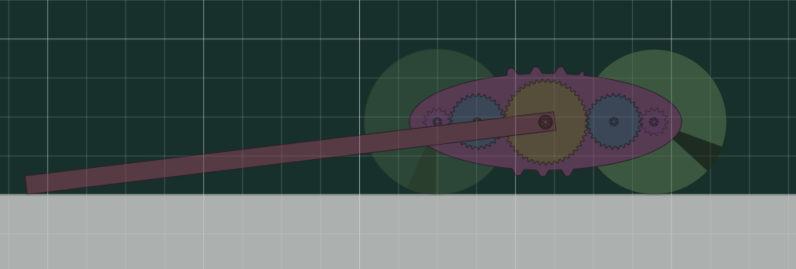
\includegraphics[width=0.8\textwidth]{algo-model2}
	\caption{Algodoo LIM system with grousers on frame}
	\label{algo-model2}
\end{figure}

\subsection{Rolling and flipping}

It was observed in simulation that the LIM would either roll or flip depending on the torque applied to it. There appeared to be a very small range of "medium torque" at which the LIM was truly load intuitive, if the motor torque was too weak it would never be able to flip over the obstacle and if it was too strong it would always flip and never roll, which hinders movement on flat terrain. However, this may simply be a result of inaccuracies of the simulation, as scaling and poor motor physics could significantly affect this motion. \\

In reality, as an electric motor increases in speed, the torque available will decrease proportionally. This means that once the LIM is rolling at speed, it will no longer have enough torque to flip itself unless it is stopped by an obstacle. This suggests that too much torque will only cause unintended flipping when the LIM is at rest on a flat plane.\\

\begin{figure}[h]
	\centering
	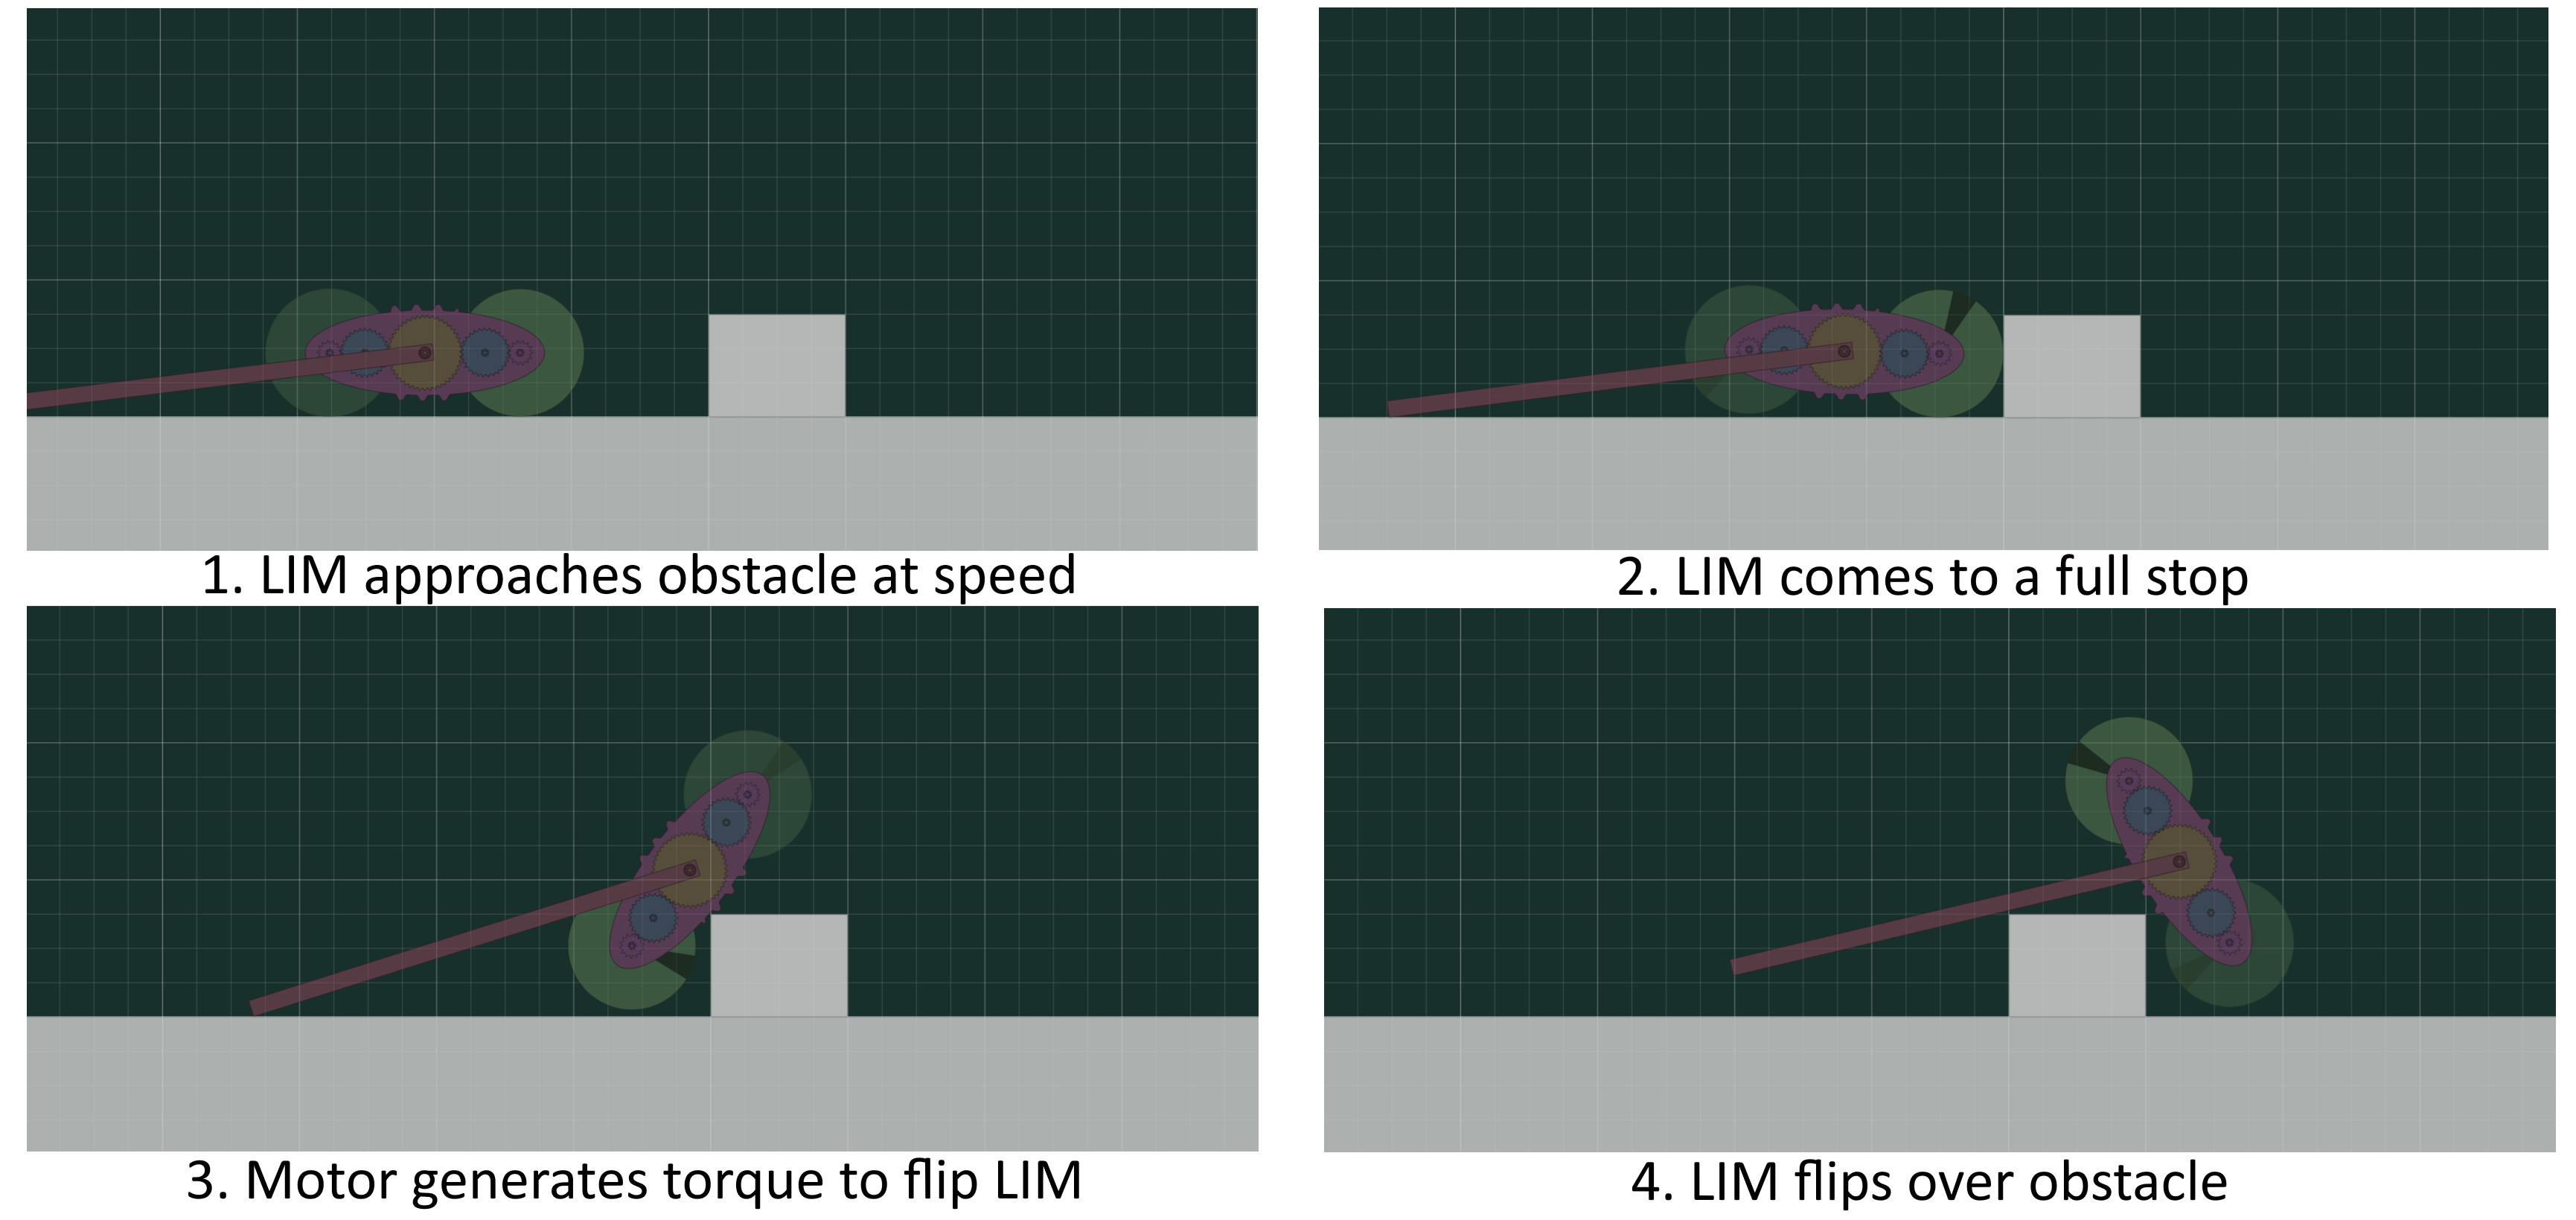
\includegraphics[width=1\textwidth]{algo-hori}
	\caption{Algodoo LIM system approaching obstacle horizontally}
	\label{algo-hori}
\end{figure}

\begin{figure}[h]
	\centering
	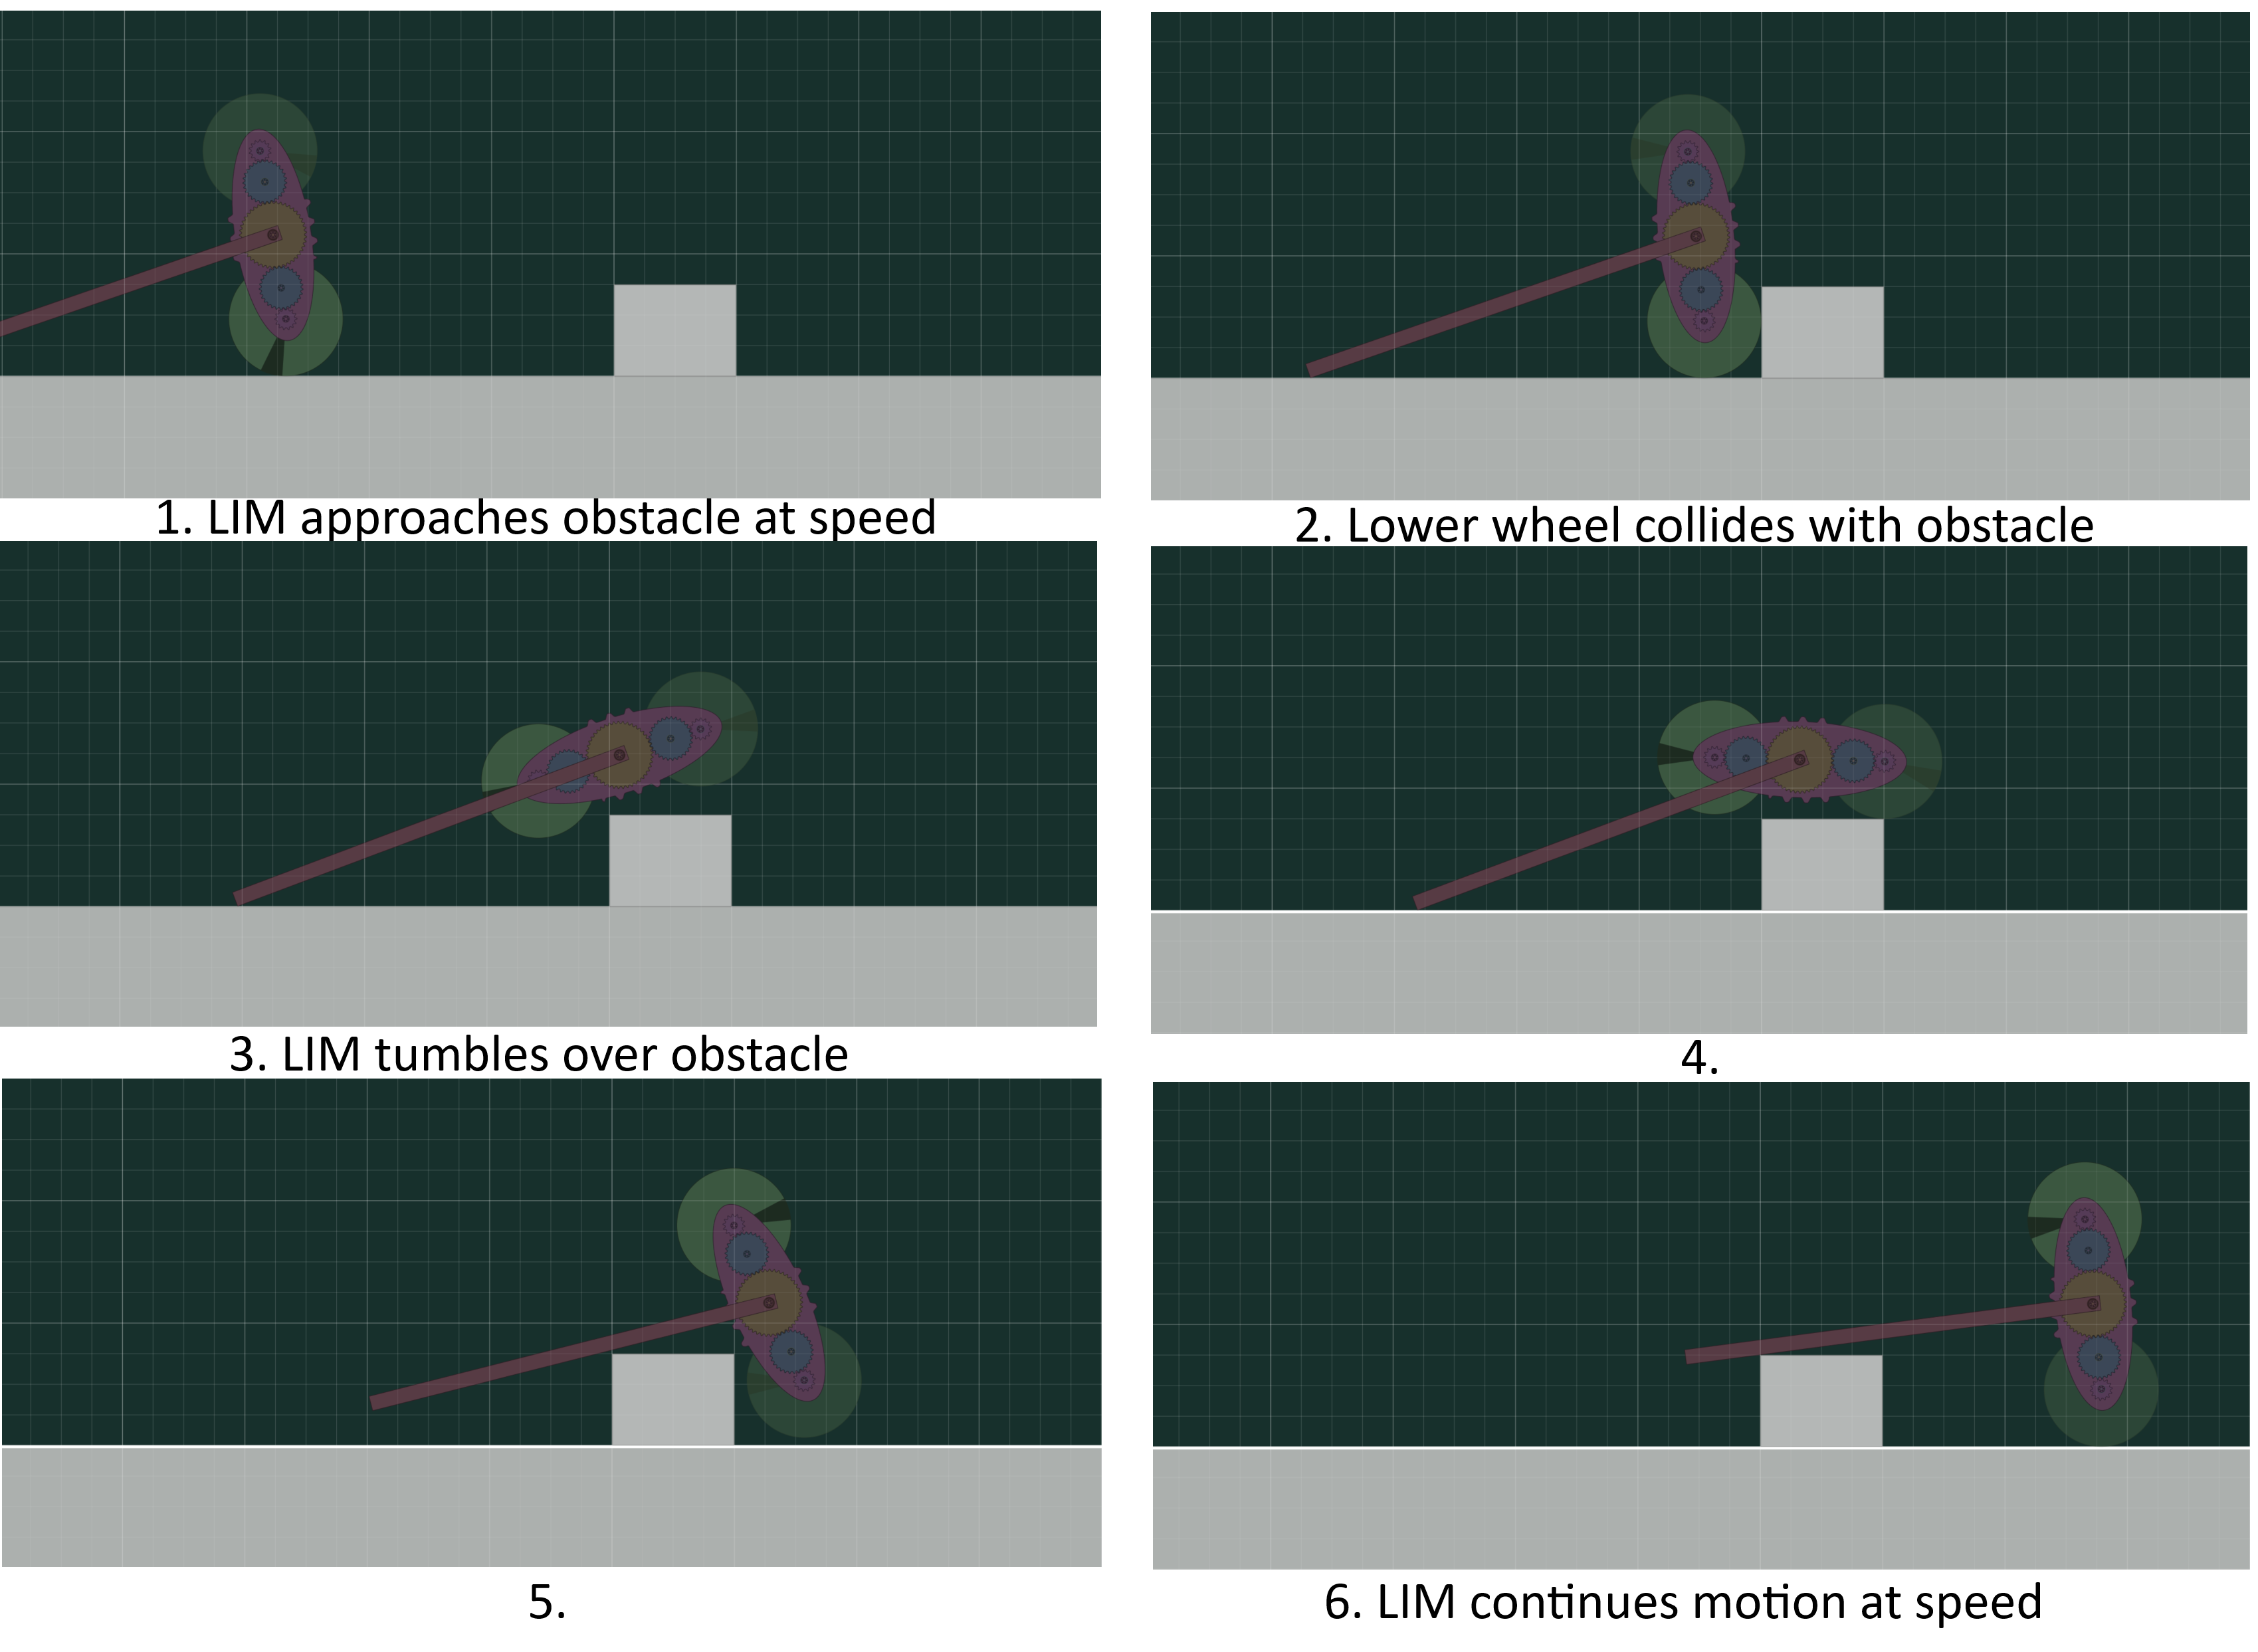
\includegraphics[width=1\textwidth]{algo-vert}
	\caption{Algodoo LIM system approaching obstacle vertically}
	\label{algo-vert}
\end{figure}

Another observation made was that if the LIM rolls at speed into the obstacle, it will have to absorb all the energy of the impact. None of the translational kinetic energy of the robot is transformed into rotational kinetic energy of the LIM for flipping. This results in quite an inefficient system. One option to mitigate this would be to implement a control system that solves the inverted pendulum problem in order to stand the LIMs upright on one wheel during normal operation. When the lower wheel encounters an obstacle while rolling, the LIM will readily flip over it without having to stop. The LIM could then switch to horizontal rolling when the robot needs a lower profile to enter a void. This solution would only be effective if a robust control system can be developed. These approaches are shown in Figures \ref{algo-hori} and \ref{algo-vert}.